% !TEX root = ../discretemath.tex

\section{Числа Рамсея}

\subsection{Определение и базовые свойства}

\begin{Definition}{Числа Рамсея}{}
	$R(m,n)$ — наименьшее натуральное число $N$ такое, что в любом простом графе на $N$
	вершинах содержится либо полный подграф на $m$ вершинах, либо независимое множество
	на $n$ вершинах.

	Эквивалентная формулировка: если рёбра полного графа $K_N$ покрасить в два цвета,
	то найдётся либо одноцветный $K_m$ первого цвета, либо одноцветный $K_n$ второго цвета.
\end{Definition}

\begin{Remark}{}{}
	Эквивалентность двух формулировок: «ребро есть / ребра нет» $\leftrightarrow$ «ребро красное / белое». Клика — это одноцветный (красный) $K_m$, независимое множество — одноцветный (белый) $K_n$.
\end{Remark}

\begin{Proposition}{}{}
	Для чисел Рамсея выполнено:
	\[
	R(1,n)=R(m,1)=1,
	\qquad
	R(m,n)=R(n,m).
	\]
\end{Proposition}

\begin{Remark}{}{}
	Симметрия $R(m,n)=R(n,m)$ — это просто обмен двух цветов местами. Равенства $R(1,n)=R(m,1)=1$ тривиальны: на одной вершине уже есть «клика $K_1$».
\end{Remark}

\begin{Example}{$R(3,3)=6$}{}
	$R(3,3)\le 6$: среди $5$ рёбер из любой вершины $v$ (в $K_6$) хотя бы $3$ одного цвета, скажем красные, ведущие в $u_1,u_2,u_3$; если какое-то ребро $u_au_b$ красное — красный треугольник с $v$, иначе $u_1u_2u_3$ — белый треугольник.

	$R(3,3)>5$: граф $K_5$ можно покрасить в два цвета без одноцветного треугольника — красные рёбра образуют пятиугольник (цикл $C_5$), белые — пентаграмму.

	\begin{center}
		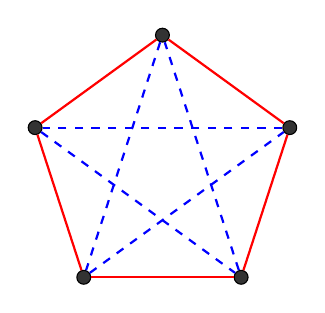
\begin{tikzpicture}[scale=1.0, font=\small,
			v/.style={circle, draw, fill=black!80, inner sep=0pt, minimum size=5pt}]
			\foreach \k in {0,...,4}{
				\node[v] (P\k) at ({90+72*\k}:1.7) {};
			}
			% пятиугольник — красные рёбра (соседние)
			\foreach \a/\b in {0/1,1/2,2/3,3/4,4/0}{
				\draw[red, thick] (P\a)--(P\b);
			}
			% пентаграмма — белые рёбра (через одну)
			\foreach \a/\b in {0/2,1/3,2/4,3/0,4/1}{
				\draw[blue, thick, dashed] (P\a)--(P\b);
			}
		\end{tikzpicture}
	\end{center}
	Ни красные (пятиугольник), ни белые (пентаграмма) рёбра не содержат треугольника, поэтому $R(3,3)>5$. Вместе с верхней оценкой $R(3,3)=6$.
\end{Example}

\subsection{Рекуррентная верхняя оценка}

\begin{Theorem}{Рекуррентная верхняя оценка}{}
	Для всех $m,n\ge 2$ выполнено
	\[
	R(m,n)\le R(m-1,n)+R(m,n-1).
	\]
\end{Theorem}

\subsubsection*{Идея доказательства}

\begin{figure}[H]
	\centering
	\begin{tikzpicture}[font=\small, >=Stealth,
		v/.style={circle, draw, fill=black!80, inner sep=0pt, minimum size=5pt}]
		\node[v,label={above:$v$}] (v) at (0,1.6) {};
		% множество X (красные рёбра)
		\draw[rounded corners, fill=red!8] (-2.7,-0.9) rectangle (-0.3,0.3);
		\node at (-1.5,-1.2) {$X$ (красные)};
		\foreach \k/\x in {1/-2.4,2/-1.9,3/-1.4,4/-0.9}{ \node[v] (xa\k) at (\x,-0.3) {}; \draw[red,thick] (v)--(xa\k);}
		% множество Y (белые рёбра)
		\draw[rounded corners, fill=blue!6] (0.3,-0.9) rectangle (2.7,0.3);
		\node at (1.5,-1.2) {$Y$ (белые)};
		\foreach \k/\x in {1/0.9,2/1.4,3/1.9,4/2.4}{ \node[v] (yb\k) at (\x,-0.3) {}; \draw[blue,thick,dashed] (v)--(yb\k);}
	\end{tikzpicture}
	\caption{Разбиение соседей вершины $v$ по цвету ребра. Если $|X|\ge R(m{-}1,n)$, то в $X$ есть красный $K_{m-1}$ (даёт с $v$ красный $K_m$) или белый $K_n$; симметрично для $Y$. Размер $N=R(m{-}1,n)+R(m,n{-}1)$ гарантирует, что одна из групп достаточно велика.}
\end{figure}

\begin{proof}
	Обозначим $N=R(m-1,n)+R(m,n-1)$ и рассмотрим любую раскраску рёбер $K_N$ в красный и белый цвета. Выберем вершину $v$; остальные $N-1$ вершин разобьём на
	\[
	X=\{u : vu \text{ — красное}\},
	\qquad
	Y=\{u : vu \text{ — белое}\}.
	\]

	\textbf{Если $|X|\ge R(m-1,n)$:} внутри $X$ найдётся либо красный $K_{m-1}$ (тогда вместе с $v$ — красный $K_m$), либо белый $K_n$ (готово).

	\textbf{Если $|Y|\ge R(m,n-1)$:} внутри $Y$ найдётся либо красный $K_m$ (готово), либо белый $K_{n-1}$ (тогда вместе с $v$ — белый $K_n$).

	Наконец, не могут одновременно выполняться $|X|\le R(m-1,n)-1$ и $|Y|\le R(m,n-1)-1$, иначе
	\[
	N-1=|X|+|Y|\le R(m-1,n)+R(m,n-1)-2=N-2,
	\]
	что невозможно. Значит, хотя бы один из двух случаев реализуется.
\end{proof}

\begin{Corollary}{Биномиальная верхняя оценка}{}
	Для всех $m,n\ge 1$ выполнено
	\[
	R(m,n)\le \binom{m+n-2}{m-1}=\binom{m+n-2}{n-1}.
	\]
\end{Corollary}

\begin{proof}[Доказательство (набросок)]
	Индукция по $m+n$ с использованием рекуррентной оценки и тождества Паскаля $\binom{a}{b}=\binom{a-1}{b-1}+\binom{a-1}{b}$; база $R(1,n)=R(m,1)=1$ согласуется с $\binom{n-1}{0}=\binom{m-1}{0}=1$.
\end{proof}

\subsection{Нижние оценки вероятностным методом}

\begin{Remark}{}{}
	Верхние оценки дают рекуррентность и биномиальная формула. Нижние оценки удобно получать вероятностным методом: показывают, что случайная раскраска $K_N$ \emph{с положительной вероятностью} не содержит запрещённых конфигураций, откуда $R(m,n)>N$. Локальная лемма Ловаса (асимметричная форма) даёт особенно хорошие нижние оценки для $R(\ell,k)$ при малом фиксированном $\ell$. В частности, этим методом получается
	\[
	R(3,k)\ge \Omega\!\left(\left(\frac{k}{\log k}\right)^2\right).
	\]
	Подробный вывод этой оценки приведён в билете о применении асимметричной локальной леммы Ловаса.
\end{Remark}
